% !TEX root = IBL-InsolvabilityOfQuintic.tex
\chapter{Solvability by Radicals}
\label{chapter:SolvabilityByRadicals}
\thispagestyle{empty}

Our overarching goal, as laid out in Chapter~\ref{chapter:PolyEquations}, is to find a polynomial whose roots can  \textbf{not} be expressed in terms of the coefficients of the polynomial using just the operations of addition, subtraction, multiplication, division, and the extraction of roots. Or, in other words, we are searching for a polynomial that is  \textbf{not} solvable by radicals, a term that we have only defined informally so far. Laying out a formal definition  of solvability by radicals (and trying to wrap our head around it) is the main goal of this chapter.


% % % % % % % % % % % % % % % % % % % % % % % % % % % % % % % % % % % % % % % % % % % %
% % % % % % % % % % % % % % % % % % % % % % % % % % % % % % % % % % % % % % % % % % % %
% SECTION
% % % % % % % % % % % % % % % % % % % % % % % % % % % % % % % % % % % % % % % % % % % %
% % % % % % % % % % % % % % % % % % % % % % % % % % % % % % % % % % % % % % % % % % % %
\begin{section}{Definition}
%Remember, when we talk about extracting roots, we must be careful to avoid ambiguous (not well-defined) notation. For this reason, we will adopt the point of view of Definition~\ref{def.nthRoot}, so $z$ being an $n^\text{th}$ root of $a$ means that $z^n = a$, as opposed to  $z = \sqrt[n]{a}$. However, we do still occasionally use the root symbol when there is no ambiguity. For example, $\sqrt[3]{5}$ and $\sqrt{-1}$ are well-defined: the first is the one and only \emph{real} solution to $x^3=5$ (although there are two other solutions in $\mathbb{C}$), and the second is $i$ (which we made a choice about long ago). However,  $\sqrt[4]{-1 + i\sqrt{3}}$ is \emph{not} well-defined, as there are $4$ equally good choices.

Our definition of solvability by radicals, needs to capture the possibility that we may need ``iterated roots'' to express a number. For example, consider \[a = \sqrt{2} + \sqrt[3]{-1 + \sqrt{2}}.\]
To see that $a$ can be expressed using addition, subtraction, multiplication, division, and the extraction of roots, we first note that the number $b = -1 + \sqrt{2}$ can be built using addition and a square root. We then arrive at $a$ by taking a cube root of $b$ and adding $\sqrt{2}$.

Let's begin to formalize this by introducing fields. Our observations above imply that $a$ can be built using field operations from $\sqrt[3]{b}$ and $\sqrt{2}$, and $b$ in turn can be built using field operations from $\sqrt{2}$. Thus, $a \in \mathbb{Q}\left(\sqrt[3]{b},\sqrt{2}\right)$ where $b \in \mathbb{Q}\left(\sqrt{2}\right)$. The lattice looks like this, where $a$ ends up in the largest field and $b$ lives in the middle field.
\begin{center}
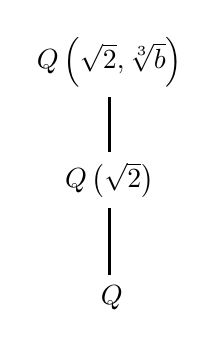
\begin{tikzpicture}[line width = 1, scale = 1.5]
\node (F2) at (0,2) {$\mathbb{Q}\left(\sqrt{2},\sqrt[3]{b}\right)$};
\node (F1) at (0,1) {$\mathbb{Q}\left(\sqrt{2}\right)$};
\node (Q) at (0,0) {$\,\mathbb{Q}$};
\draw (Q) -- (F1);\draw (F1) -- (F2);
\end{tikzpicture}
\end{center}

We are close to the definition, but first, a word of caution. When we talk about extracting roots, we must be careful to avoid ambiguous (not well-defined) notation. For this reason, we will adopt the point of view of Definition~\ref{def.nthRoot}, so $z$ being an $n^\text{th}$ root of $a$ means that $z^n = a$, as opposed to  $z = \sqrt[n]{a}$. That said, we do still occasionally use the root symbol when there is no ambiguity. For example, $\sqrt[3]{5}$ and $\sqrt{-1}$ are well-defined: the first is the one and only \emph{real} solution to $x^3=5$ (although there are two other solutions in $\mathbb{C}$), and the second is $i$ (which we made a choice about long ago). However,  $\sqrt[4]{-1 + i\sqrt{3}}$ is \emph{not} well-defined, as there are $4$ equally good choices.

\begin{definition}
Let $F$ be a field. We say  $E$ is a \textbf{radical extension} of $F$ if there exist nonzero elements $r_1,r_2,\ldots,r_m\in E$ and positive integers $n_1,n_2\ldots,n_m$ such that $E = F(r_1,r_2,\ldots,r_m)$, and 
\begin{align*}
 r_1^{n_1} &\in F,\\
 r_2^{n_2} &\in F(r_1),\\
 r_3^{n_3} &\in F(r_1,r_2),\\
 \vdots & \\
 r_k^{n_k} &\in F(r_1,\ldots,r_{k-1}).
\end{align*}
\end{definition}
Notice that the final condition of the definition expresses that each $r_i$ is an $n_i^\text{th}$-root of some element in $F(r_1,\ldots,r_{i-1})$. 

When $a = \sqrt{2} + \sqrt[3]{-1 + \sqrt{2}}$, our work above shows  $a$ is contained in  $E= \mathbb{Q}\left(\sqrt{2},\sqrt[3]{-1 + \sqrt{2}}\right)$ and $E$ is a radical extension of $\mathbb{Q}$, since we may take $r_1 = \sqrt{2}$ and $r_2 = \sqrt[3]{-1 + \sqrt{2}}$ (with $n_1 = 2$ and $n_2 = 3$).


%\begin{problem}
%Show that $\mathbb{Q}\left(\sqrt{2},\sqrt[3]{-1 + \sqrt{2}}\right)$
%\end{problem}
%
%\begin{problem}
%Let $p(x) = x^4+3x^2+1$.  Find the four roots of $p(x)$ and explain how each root can be built using addition, subtraction, multiplication, division, and roots (and all rational numbers) 
%\end{problem}


\end{section}








